\documentclass[11pt]{article}
\usepackage{amsmath}
\usepackage{geometry}
\usepackage{graphicx}
\usepackage{array}
\usepackage{multicol}

\geometry{a4paper, top=0.5in, bottom=0.5in, right=0.75in, left=0.75in}

\title{Power}
\author{Abanoub Emad Hanna}
\date{}

\begin{document}

\maketitle
\section*{Introduction}
\begin{itemize}
    \item The focus should be \textbf{Energy-Efficiency} rather than Low-Power, because batteries provide energy not power. For example, if you have a slow low power device but needs multiple cycles to do a given operation, it would end up consuming more power than a fast high power device.
    \item Capacitors don't dissipate energy, they store it. However, the charging or discharging of capacitors consume energy in form of heat lost in PMOS \& NMOS.
\end{itemize}

\section*{Static Power}
\subsection*{Leakage Power}
\begin{itemize}
    \item Power consumed when there is no transition or device is idle.
    \item Main sources of leakage power are:
        \begin{itemize}
            \item \textbf{Subthreshold Leakage:} It is the main source and happens when $V_{WI}<V_{gs}<V_{th}$ ($V_{WI}$ is the weak inversion voltage). Current flows exponentially with $V_{th}$.
            \item \textbf{Gate Leakage:} Current flows through the gate oxide due to tunneling of electrons in presence of high electric field \& thin oxide.
            \item \textbf{Contention Current:} Current flows when a node is driven by multiple sources with different values.
        \end{itemize}
\end{itemize}

\section*{Dynamic Power}
\subsection*{Switching Power}
\begin{itemize}
    \item The power dissipated during charging and discharging of load capacitors.
    \item For a single transition, energy drawn from supply is $E_{V_{DD}}=C_LV_{DD}^2$; half that energy is stored in the capacitor and the other half is dissipated in the PMOS or NMOS. Therefore:
    \begin{equation*}
        P_{\text{switching}}=\alpha f_{\text{clk}}C_LV_{DD}^2
    \end{equation*}
    where $\alpha=0.5$ for all signals \& 1 for clock signals (2 transitiosn per cycle).
\end{itemize}
\subsection*{Glitching Power}
\begin{itemize}
    \item We can consider it a subcomponent of switching power.
    \item Glitches occur due to different arrival times of signals at a multi-input gate due to different path delays.
    \item Glitches ripple through the circuit and increase the activity factor.
\end{itemize}
\subsection*{Short-Circuit Power}
\begin{itemize}
    \item The power dissipated during the short-circuit current that flows through the PMOS and NMOS when they are both on ($V_{th} < V_{in} < V_{DD}-V_{th}$).
    \item Mainly affected by the rise/fall times of the signals as well as $V_{th}/V_{DD}$ ratio.
    \item It can be ignored if $V_{th}=0.5V_{DD}$ (nanometer technologies).
\end{itemize}

\section*{Power Reduction Techniques}
\subsection*{Activity Factor Reduction}
\subsubsection*{Clock Gating}
The best way to reduce the activity is to turn off the clock to registers in unused blocks.
\begin{itemize}
    \item \textbf{Latch-Free:} Gated clock is generated by EN AND CLK. However, this is a very bad design because:
        \begin{itemize}
            \item EN glitchs would cause multiple rising edges for the same clock cycle.
            \item \textbf{Pulse Clipping:} Falling transition for EN signal when clock is high, which leads to pulse width violation.
            \item \textbf{Spurious Clocking:} Rising transition for EN signal when clock is high, which leads to timing violation.
        \end{itemize}
        \begin{multicols}{2}
            \begin{minipage}{\linewidth}
                \begin{center}
                    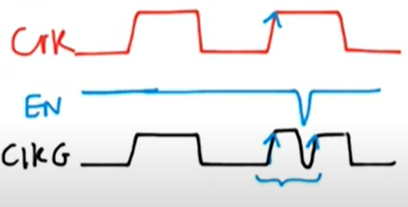
\includegraphics[width=0.8\textwidth]{1.png}
                \end{center}
            \end{minipage}
            \begin{minipage}{\linewidth}
                \begin{center}
                    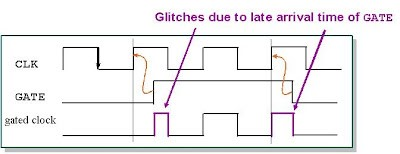
\includegraphics[width=1\textwidth]{2.jpeg}
                \end{center}
            \end{minipage}
        \end{multicols}
    \item \textbf{Latch-Based:} This method uses a negative latch (for positive-edge triggered FF) to ensure that enable signal can only change when the clock is low. However, this method introduces clock skew which can cause spurious clocking, so a special cell is used (Integerated Clock Gating Cell).
        \begin{center}
            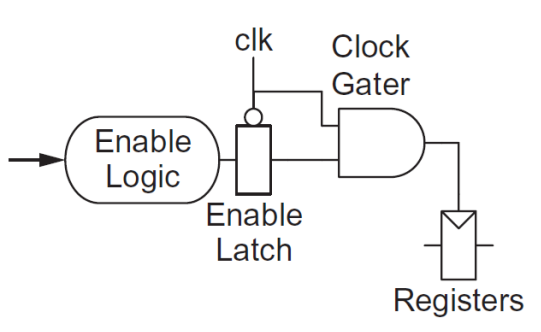
\includegraphics[width=0.5\textwidth]{3.png}
        \end{center}
\end{itemize}
\textbf{Important Notes:}
\begin{itemize}
    \item Clock gating is only applicable if EN signal is expected to be low for a long time.
    \item Clock gating block should be placed close to the clock source to avoid clock skew.
\end{itemize}

\subsubsection*{Other Techniques}
\begin{itemize}
    \item \textbf{Operand Isolation:} Registering inputs help avoid glitches. However, it increases the area and add latency of 1 clock cycle.
    \item Avoid using XOR because it has a high activity factor (0.5 instead of 0.25).
    \item Avoid comparisons ($ <, >$) because they involve many XORs.
    \item Use shifters instead of multipliers; multipliers have a huge area consume a lot of power.
\end{itemize}

\subsection*{Frequency Reduction}
Run each block at the lowest possible frequency that meets performance requirements by using clock dividers.

\subsection*{Voltage Reduction}
\begin{itemize}
    \item Use multiple voltage domains (different $V_{DD}$) for each block.
    \item However, level converters (shifters) are required when crossing different voltage domains. This is to account for the different noise margins. For example, a 1V signal has a noise margin of 0.5V for 1V domain, but 0.1 for 1.8V domain.
\end{itemize}
 
\subsection*{Short Circuit (\& Leakage) Power Reduction}
\begin{itemize}
    \item Use multiple threshold voltages. The higher the threshold voltage, the lower the power.
    \item However, this increases the delay, so we start with high threshold voltage cells and introduce low threshold voltage cells for critical paths.
\end{itemize}

\section*{Power Gating}
\begin{itemize}
    \item Power gating is used to turn off the power supply to a block when it is not in use through a high $V_{th}$ PMOS switch controlled by Power-EN signal.
    \item The power gating block should use special FF cells called Retention FF to prevent data loss.
    \item \textbf{Retention Flops:} 
        \begin{itemize}
            \item They hold their internal state when the primary power supply is shut down and restore the state when the power is brought up. 
            \item They use Always-On power supply for slave latches only.
        \end{itemize}
    \item If a block's input is from a power-gated block, this input will be floating causing short circuit current. To avoid this, we use isolation cells to drive the input to ground during off state.
\end{itemize}
\begin{center}
    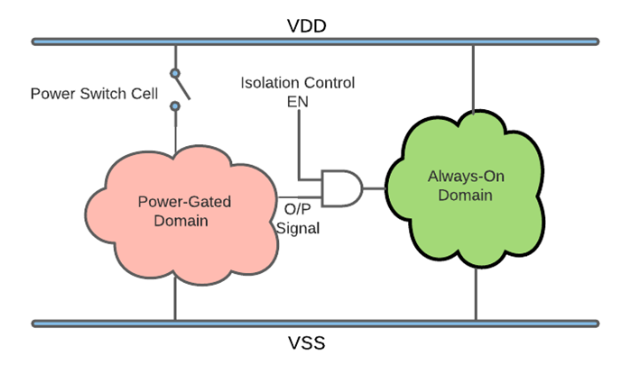
\includegraphics[width=0.7\textwidth]{4.png}
\end{center}

\end{document}